\subsection{Biblioteki pomocniczne}
Podczas pracy z projektem zostały wykorzystane popularne biblioteki ułatwiające podstawowe zadania. Wszystkie z nich są darmowe nawet w wykorzystaniu komercyjnym oraz całkowicie otwarte.
\begin{enumerate}
  \item jQuery --- lekka biblioteka ułatwijąca operacje na elementach DOM i ułatwiająca pracę z językiem Javascript.
  \item jQuery-UI --- plugin do biblioteki jQuery umożliwiający tworzenie zaawansowanych wizualnych elementów, takich jak okna dialogowe, elementy rozszerzalne (ang. resizable), elementy przesuwalne (ang. draggable).
  \item jQuery-mousewheel --- plugin do biblioteki jQuery dodający obsługę kółka myszy.
  \item sylvester.js --- biblioteka służąca do zaawansowanych obliczeń na macierzach i wektorach.
\end{enumerate}


\subsection{Połączenie}
Klient po załadowaniu początkowej strony dokonuje połączenia WebSocket z serwerem na port podany na stronie. Następnie nasłuchuje na informacje od serwera i na każdą z nich reaguje. Komunikaty w formacie JSON w drugą stronę wysyłane są po zajściu zdarzeń po stronie klienta, np. ruchu myszą. Dokładny opis zdarzeń znajduję się w sekcji \ref{client_events}.

\subsection{Window manager (ang. zarządca okien)}
Typowe programy komputerowe składaja się z wielu okien. Sposób implementacji pseudookien i zarządcy w projekcie był możliwy na dwa sposoby.
Pierwszym wariantem jest zastosowanie osobnych okien przeglądarki (tzw. popupów), które odpowiadałyby rzeczywistym oknom przeglądarki.
Drugą opcją jest stworzenie minimalistycznego managera okien w języku Javascript.

Główną wadą rozwiązania jest całkowitym brak możliwości sterowania oknami. Przeglądarka nie jest w stanie zablokować możliwości zamknięcia okna, sterować ich modalnościa oraz przyciskami sterowania (minimalizacji, maksymalizacji, zamknięcia i innymi). Co więcej stosowanie dodatkowych okien przeglądarki jest uważane za złą praktykę.

Z powodu tak dużej ilości problemów w projekcie zdecydowano się na użycie drugiego wariantu. Do stworzenia okien wykorzystana została biblioteka jQuery-UI dostarczająca metody umożliwiający w przystępny sposób tworzenie elementów rozszerzalnych (ang. resizable) oraz przeciągalnych (ang. draggable). Celem funkcjonalnym było upodobnienie zachowania pseudookien w przeglądarce do prawdziwych okien programu:
\begin{itemize}
  \item zmiana rozmiaru okna przy pomocy uchwytów w rogach i na krawędziach,
  \item przenoszenie okien za pomocą paska tytułowego,
  \item minimalizacja, maksymalizacja oraz zamykanie okien za pomocą przycisków w prawym górnym rogu.
\end{itemize}

Okno na stronie jest elementem blokowym typu \emph{div} z zagnieżdżonymi elementami symulującymi swoje odpowiedniki z systemowego menedżera okien.
Rysunki \ref{fig:modal} i \ref{fig:non_modal} przedstawiają menedżer okien wyświetlający okno w trybie modalnym oraz niemodalnym.

\begin{figure}
\centering
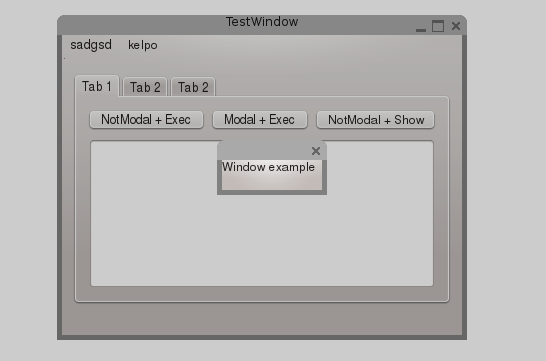
\includegraphics[width=0.7\linewidth]{img/modal}
\caption{Okno modalne -- obszar za oknem jest zacieniowany i niedostępny.}
\label{fig:modal}
\end{figure}

\begin{figure}
\centering
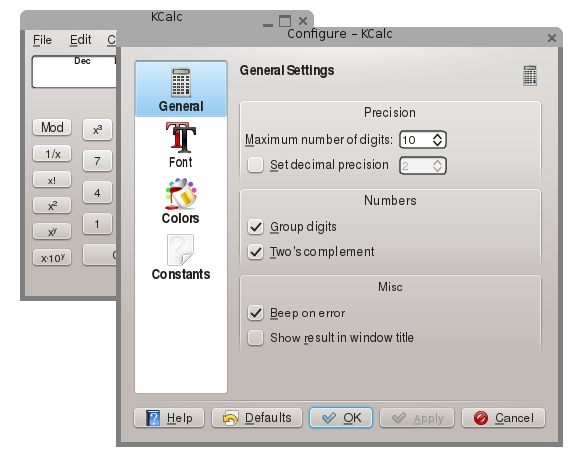
\includegraphics[width=0.7\linewidth]{img/non_modal}
\caption{Okno niemodalne -- obszar za oknem jest dostępny.}
\label{fig:non_modal}
\end{figure}


Zaimplementowana funkcjonalność maksymalizacji okna po stronie przeglądarki różni się od funkcjonalności w rzeczywistym środowisku (po stronie serwera). Maksymalizacja polega na zwiększeniu rozmiarów okna do maksymalnego dostępnu obszaru na stronie HTML.
Takie rozwiązanie wynika z możliwości uruchomienia serwera aplikacji w serwerze X11 w dowolnej rozdzielczości. Po faktycznym zmaksymalizowaniu okna na serwerze użytkownik po stronie przeglądarki widziałby okno o rozmiarze innym niż pełny dostępny obszar widoku w przeglądarce. W przypadku rozmiaru mniejszego skutkowałoby to pustym, niezagospodarowanym miejscem w oknie przeglądarki, natomiast większy rozmiar powodowałby pojawienie się suwaków przewijania (ang. scrollbar).

Funkcjonalność minimalizacji okna jest również symulowana. Okno jest chowane poprzez zmianę wartości CSS \emph{display} na \emph{none}. Dodatkowo tworzony jest element na pasku zadań, który po kliknięciu przywraca ukryte okno. Pasek zadań jest elementem strony znajdującym się na samym dole. Przykładowy pasek z jedną zminimalizowaną aplikacją przedstawia rysunek \ref{fig:taskbar}

\begin{figure}
\centering
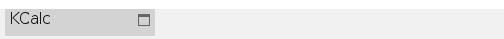
\includegraphics[width=0.7\linewidth]{img/taskbar}
\caption{Przykładowy pasek zadań z aplikacją \emph{KCalc}}
\label{fig:taskbar}
\end{figure}


\subsection{Rysowanie pojedynczego widgeta}
Widget reprezentowany jest przez element \emph{div} zawierający dwa elementy: element \emph{canvas} oraz kontener \emph{div} na widgety potomne posiadające analogiczną struktruę. Element ten ma pełni funkcję pomocniczą (jest w pełni przeźroczysty) i służy do umiejscowienia elementu w stosounku do jego rodzica za pomocą atrybutów CSS \emph{left} oraz \emph{top}. Taka implementacja relacji rodzic-dziecko widgetów na stronie zapewnia drzewiastość i łatwość zarządzania widgetami. Zmiana rodzica widgeta, który posiada zagnieżdzone dzieci nie jest problematyczna, a ze względu na format przesyłanych danych od serwera ta operacja jest bardzo często używana na etapie tworzenia okien.
Widgety z flagą \emph{Qt::Window}, czyli przede wszystkim dziedziczące z \emph{QDialog} oraz \emph{QMainWindow} są traktowane w specjalny sposób. Są opakowywane w kontener okna opisany powyżej i są elementami stojącymi najwyżej w strukturze drzewa.

\begin{figure}
\centering
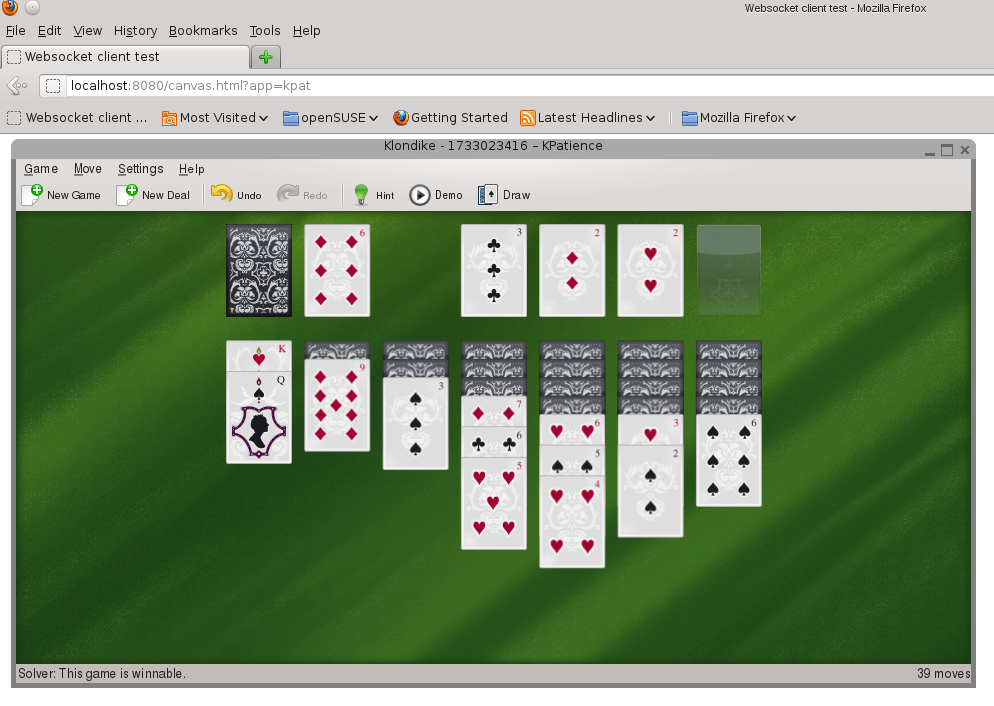
\includegraphics[width=0.7\linewidth]{img/example}
\caption{Przykład skomplikowanej aplikacji \emph{KPatience} z wieloma widgetami uruchomionej w przeglądarce \emph{Mozilla Firefox}.}
\label{fig:example}
\end{figure}
